%%%%%%%%%%%%%%%%%%%%%%%%%%%%%%%%%%%%%%%%%%%%%%%%%%%%%%%%%%%%%%%%%%%%
%% I, the copyright holder of this work, release this work into the
%% public domain. This applies worldwide. In some countries this may
%% not be legally possible; if so: I grant anyone the right to use
%% this work for any purpose, without any conditions, unless such
%% conditions are required by law.
%%%%%%%%%%%%%%%%%%%%%%%%%%%%%%%%%%%%%%%%%%%%%%%%%%%%%%%%%%%%%%%%%%%%

\documentclass[
  digital, %% This option enables the default options for the
           %% digital version of a document. Replace with `printed`
           %% to enable the default options for the printed version
           %% of a document.
  notable,   %% Causes the coloring of tables. Replace with `notable`
           %% to restore plain tables.
  nolof,     %% Prints the List of Figures. Replace with `nolof` to
           %% hide the List of Figures.
  nolot,     %% Prints the List of Tables. Replace with `nolot` to
           %% hide the List of Tables.
  nocover
  %% More options are listed in the user guide at
  %% <http://mirrors.ctan.org/macros/latex/contrib/fithesis/guide/mu/fi.pdf>.
]{fithesis3}
%% The following section sets up the locales used in the thesis.
\usepackage[resetfonts]{cmap} %% We need to load the T2A font encoding
\usepackage[T1,T2A]{fontenc}  %% to use the Cyrillic fonts with Russian texts.
\usepackage[
  main=english, %% By using `czech` or `slovak` as the main locale
                %% instead of `english`, you can typeset the thesis
                %% in either Czech or Slovak, respectively.
  english,czech %% The additional keys allow
]{babel}        %% foreign texts to be typeset as follows:
%%
%%   \begin{otherlanguage}{german}  ... \end{otherlanguage}
%%   \begin{otherlanguage}{russian} ... \end{otherlanguage}
%%   \begin{otherlanguage}{czech}   ... \end{otherlanguage}
%%   \begin{otherlanguage}{slovak}  ... \end{otherlanguage}
%%
%% For non-Latin scripts, it may be necessary to load additional
%% fonts:
\usepackage{paratype}
\def\textrussian#1{{\usefont{T2A}{PTSerif-TLF}{m}{rm}#1}}
%%
%% The following section sets up the metadata of the thesis.
\thesissetup{
    date          = \the\year/\the\month/\the\day,
    university    = mu,
    faculty       = fi,
    type          = mgr,
    author        = Martina Vitovská,
    gender        = f,
    advisor       = {doc. RNDr. Jan Strejček, Ph.D.},
    title         = {Instrumentation of LLVM IR},
    TeXtitle      = {Instrumentation of LLVM IR},
    keywords      = {instrumentation, verification, static analysis, LLVM, ...},
    TeXkeywords   = {instrumentation, verification, static analysis, LLVM, \ldots},
    abstract      = {This is the abstract of my thesis, which can span multiple paragraphs.},
    thanks        = {These are the acknowledgements for my thesis, which can span multiple paragraphs.},
}

\usepackage{caption}
\newcommand{\thenalg}{\thechapter .\arabic{nalg}}
\DeclareCaptionLabelFormat{algocaption}{Algorithm \thenalg} % defines a new caption label as Algorithm x.y

\usepackage[backend=biber]{biblatex}
\addbibresource{references.bib}

\usepackage{makeidx}      %% The `makeidx` package contains
\makeindex                %% helper commands for index typesetting.
%% These additional packages are used within the document:
\usepackage{paralist} %% Compact list environments
\usepackage{amsmath}  %% Mathematics
\usepackage{amsthm}
\usepackage[table]{xcolor}
\usepackage{amsfonts}
\usepackage{url}      %% Hyperlinks
\usepackage{listings} %% Source code highlighting
\lstset{
  basicstyle      = \ttfamily,%
  identifierstyle = \color{black},%
  keywordstyle    = \color{blue},%
  keywordstyle    = {[2]\color{cyan}},%
  keywordstyle    = {[3]\color{olive}},%
  stringstyle     = \color{teal},%
  commentstyle    = \itshape\color{magenta}}
\usepackage{floatrow} %% Putting captions above tables
\floatsetup[table]{capposition=top}

\usepackage{tikz}
\usetikzlibrary{shapes,arrows}
\usepackage{smartdiagram}
\usesmartdiagramlibrary{additions}
\usepackage{styles/llvm}
\usepackage{styles/nasm}

\usepackage{xspace}
\usepackage{xcolor}
\usepackage{subcaption}

\newcommand{\todo}[1]{\textcolor{red}{#1}}
\newcommand{\llvm}{\textsc{llvm}\xspace}
\newcommand{\symbiotic}{\textsc{Symbiotic}\xspace}
\newcommand{\klee}{\textsc{Klee}\xspace}
\newcommand{\stacklist}{\texttt{stack\_list}\xspace}
\newcommand{\globalslist}{\texttt{globals\_list}\xspace}
\newcommand{\heaplist}{\texttt{heap\_list}\xspace}
\newcommand{\dealloclist}{\texttt{deallocated\_list}\xspace}
\newcommand{\llvmpin}{\textsc{LLVMPin}\xspace}
\newcommand{\clang}{\textsc{Clang}\xspace}

\lstnewenvironment{algorithm}[1][] %defines the algorithm listing environment
{
    \refstepcounter{nalg} %increments algorithm number
    \captionsetup{labelformat=algocaption,labelsep=colon} %defines the caption setup for: it ises label format as the declared caption label above and makes label and caption text to be separated by a ':'
    \lstset{ %this is the stype
        mathescape=true,
        frame=lines,
        numbers=left,
        numberstyle=\tiny,
		numbersep=5pt,
        basicstyle=\footnotesize,
        keywordstyle=\color{black}\bfseries,
        keywords={,input, output, return, datatype, in, if, else, foreach, while, begin, end, then,and, or, }
        numbers=left,
        xleftmargin=1em,
		framexleftmargin=1em,
        #1 % this is to add specific settings to an usage of this environment (for instnce, the caption and referable label)
    }
}
{}

\begin{document}
\chapter{Introduction}
As our lives became highly dependent on computers, the question of software
reliability turned to be a serious issue. If we take into consideration the
size and the complexity of today's computer programs, it is almost impossible
to find bugs in a code manually. The need for automatic program analysis is
therefore increasing.

We can distiguish two types of program analysis: dynamic and static. Whereas
dynamic analysis is performed by executing the program, static analysis
inspects a representation of a program (e.g. a source code) and analyzes it
without actually running it.

One of the techniques used for both dynamic and static program analysis is
instrumentation. Instrumenting a program means inserting a new code into an
existing code in order to gather information relevant for program analysis. The
new code usually does not change the behaviour of the program. Instrumentation
is for example used in profilers which insert instructions for gathering
information about time or memory consumption. It is also used by many tools
that check memory safety of programs as it is possible to track the state of
the memory with the inserted code.

The aim of this thesis is to present an overview of existing tools for
instrumentation of LLVM IR bitcode and to design a new tool for
instrumentation of LLVM IR. The tool should be configurable and should offer the
possibility to use results of external static analyses to reduce the amount of
newly inserted code. Another goal is to create a configuration for finding
memory safety errors such as double free, invalid dereference or
use-after-free-error.

The new tool is implemented as an independent module, which means it can be
incorporated in any tool that performs the actual analysis on the instrumented
program. We employed the instrumentation in \symbiotic~\cite{Symbiotic} which
is an open-source tool for static analysis of sequential programs in LLVM. It
uses three techniques for static analysis: instrumentation, program slicing and
symbolic execution. Instrumentation in \symbiotic is used to reduce the problem
of checking some property violations (e.g. checking for NULL pointer
dereference) to a reachability problem. In other words, a given program is
instrumented such that the original program violates the property if and only
if some error location is reachable in the instrumented program. Program
slicing~\cite{weiser} is a technique that removes a code that is not
relevant for the reachability of error locations, therefore the actual
analysis is performed on a smaller amount of code and is consequently
faster. The sliced program is passed to a symbolic executor~\cite{King} that goes
through every possible path of a program (if the program terminates)
because it uses symbolic values instead of the real values. The executor than
looks whether some error location is reachable.


Chapter~\ref{chap:tools} lists the existing tools for instrumenting LLVM IR and
tools that use instrumentation of LLVM IR for analysis of programs and
discusses their benefits and drawbacks.

In Chapter~\ref{chap:instr} the general approach of our configurable
instrumentation is described together with the configuration files that must
be provided.

Chapter~\ref{chap:memsafety} deals with a configuration of instrumentation for
checking memory safety errors. Besides the basic approach, we also propose an
enhancement with a pointer analysis and with staged instrumentation to make the
whole verification process faster.

In Chapter~\ref{chap:eval} we show evaluation of instrumentation designed for
memory safety implemented in \symbiotic. We compare the enhancements on a
set of benchmarks from
SV-COMP~\footnote{\url{https://sv-comp.sosy-lab.org/2017/benchmarks.php}}.

Chapter~\ref{chap:conclusion} is a conclusion of this thesis.

\todo{future work}


\chapter{LLVM}\label{chap:llvm}
\url{www.aosabook.org/en/llvm.html}
\medskip

LLVM is an open source project that provides compiler technologies designed to
be independent of a target architecture. It uses LLVM IR as an intermediate
representation code. It can be used in three different forms: human readable
representation, bitcode representation and an in-memory compiler IR. From this
point we will take only the human readable form into consideration for the sake
of simplicity.

\begin{figure}[h]
 \lstinputlisting[language=llvm,style=nasm]{examples/llvm.ll}
 \caption{Example of an LLVM module with function \texttt{main} that calls
 \texttt{foo} function which allocates an array of ten integers and stores
 \texttt{number} in the first field of the array.}
 \label{fig:llvm_example}
\end{figure}

\section{LLVM structure} %TODO rename the chapter to LLVM IR?

The high-level structure of an LLVM program consists of modules, which are
units created when a program is translated. More modules can be linked together
with the LLVM linker. These units contain global variables and functions.

Each function begins with a \texttt{define} keyword and is composed of basic
blocks. Basic blocks are sequences of instructions and have a single entry node
and a single exit node, i.e. there is no branching in a basic block. They form
a control flow graph for a function. In figure~\ref{fig:llvm_example} we give
an example of an LLVM module with two function definitions, each containing one
basic block.

LLVM is in SSA form (static single assignment form), which means that each
variable can be assigned only once and must be defined before its use. It uses:

\begin{itemize}
    \item global identifiers that begin with the '@' character for functions
    and global variables, for example global variable \texttt{@number} in
    figure~\ref{fig:llvm_example}, and
    \item local identifiers that begin with the '\%' character for register
    names and types, for example a local variable \texttt{\%a} in
    figure~\ref{fig:llvm_example}.
\end{itemize}

Both kinds of identifiers can be named or unnamed, unnamed identifiers are
represented as unsigned numeric values (e.g. local identifier \texttt{\%1} in
figure~\ref{fig:llvm_example}).

\section{LLVM types}

LLVM is a strongly typed language, i.e. all values and variables are typed.
There are simple types such as integer type (e.g. \texttt{i32} for a 32-bit
integer), floating point types (e.g. \texttt{float} or \texttt{double}) and
pointer type (e.g. \texttt{i32*} for a pointer to a 32-bit integer), and also
types for vectors (e.g. \texttt{<10 x i32>} for a vector of 10 32-bit
integers), arrays (e.g. \texttt{[10 x i32]} for an array of 10 32-bit integers)
and structures (e.g. \texttt{\{i32, i32\}} for a pair of 32-bit integers). For
example, in figure~\ref{fig:llvm_example} we can see that global variable
\texttt{number} is a 32-bit integer and \texttt{a} is an array of ten
32-bit integers.

\section{Basic instructions}

There are five classes of LLVM instructions: terminator instructions, binary
instructions, bitwise binary instructions, memory instructions and other
instructions.

A terminator instruction is used as the last instruction of each basic block
and it determines which block will follow after the current one. For our
purposes we will describe only two of the terminator instructions: \texttt(ret)
and \texttt{br}.

\texttt{ret} instruction is used to return from a function to a basic block
from which the function was called. It has one optional argument that represent
a return value of a function. In figure~\ref{fig:llvm_example} we can see the
two variants of this instruction: in function \texttt{foo}, there is a
\texttt{ret void} instruction, because this function does not return any value,
whereas function \texttt{main} returns 0 (\texttt{ret i32 0}).

\texttt{br} instruction determines which basic block from the current function
will follow. It represents either conditional branching \texttt{br i1
<condition>, label <true-branch>, label <false-branch>} transfering the control
flow to \texttt{true-branch} block if the \texttt{condition} holds and to
\texttt{false-branch} block otherwise, or uncoditional branching \texttt{br
label <b>} transfering the control flow to a block \texttt{b} unconditionally.

Binary operator instructions have two operands of the same type and return a
result of an operation on these operands, for example \texttt{add} instruction
for addition or \texttt{sub} instruction for subtraction. There are usually two
versions of these instructions: one for integer values and one for floating
point values. These instructions together with bitwise binary instructions
that are used for bitwise operations are not relevant for this work.

The two most important instructions for working with memory are \texttt{load}
and \texttt{store}. \texttt{load} instruction is used to read from memory
specified by its operand, whether \texttt{store} is used to write to memory and
has two operands: a value to store and address of a target memory. We can see
the usage of \texttt{load} and \texttt{store} in figure~\ref{fig:llvm_example}
in function \texttt{foo} where a value of global variable \texttt{number} is
read, marked as \texttt{\%1} and later stored to \texttt{\%2}. Another
instruction relevant for our work is \texttt{alloca} instruction for allocating
memory on the stack. In figure~\ref{fig:llvm_example}, in function \texttt{foo}
\texttt{alloca} instruction is used to allocate \texttt{a} as an array of ten
32-bit integers on the stack. Instruction \texttt{getelementptr} gets the
address of some element of an aggregate data structure, for example in
figure~\ref{fig:llvm_example} in function \texttt{foo} it gets the address of
the fifth element of array \texttt{a}.

Relevant instruction from the category of other instructions is \texttt{call}
which calls a function given as its operand together with function's arguments.
We can find an example of a \texttt{call} instruction in
figure~\ref{fig:llvm_example} in function \texttt{main} which calls function
\texttt{foo} on line~15.


\chapter{Overview of Existing Tools}\label{chap:tools}
In this chapter, we list tools that work with instrumentation of LLVM. In the
first section, we describe a framework for general instrumentation where the
user is somehow able to control the instrumentation in terms of what
instructions will be inserted, etc. In the second section, we list the tools
that use the instrumentation for specified purposes such as checking memory
safety.

\section{LLVMPin Instrumentation Framework}\label{sec:llvmpin}

\llvmpin~\cite{llvmpin} is a framework that simplifies implementing tools for
instrumentation of LLVM~IR. First of all, a user has to implement
an~\textsc{LLVMPin} tool, which is a C++ code that must contain three parts:

\begin{itemize}
    \item Analysis part that contains definitions of analysis functions and a
    routine for analysis setup. Analysis functions are functions that can be
    inserted into the given code to perform an analysis of the program.
    \item \texttt{INSTRUMENT} routine that inserts calls to analysis functions
    defined by user.
    \item \texttt{REQUIRE} routine with a list of existing LLVM
    passes\footnote{\url{http://llvm.org/docs/WritingAnLLVMPass.html}} required
    by the \textsc{LLVMPin} tool.
\end{itemize}

The framework basically consists of two scripts:

\begin{itemize}
    \item \texttt{llvmpin-gen} compiles the \textsc{LLVMPin} tool,
    \item \texttt{llvmpin} runs the instrumentation, gerates the new bitcode
    and from the bitcode it produces an executable.
\end{itemize}

The framework comes with the API that provides several functions and macros
that are useful for the instrumentation, for example a function
\texttt{INS\_InsertCall} that adds a call to an analysis function. However, a
user still has to implement the eintire \texttt{INSTRUMENT} routine to describe
how to instrument the code, including the procedure that searches for the
instructions that should be instrumented.

To summarize, the \textsc{LLVMPin} framework is one of a few instrumentation
tools for LLVM IR that are general and configurable, but it does not simplify
the work for the user in terms of writing a code that performs the core of the
instrumentation process.

\section{Other Tools}

In this section, we describe tools that are not designed for general
instrumentation but use instrumentation over LLVM for various purposes.

\textsc{Clang} compiler (licensed under University of Illinois/NCSA Open Source
License) provides several sanitizers that use instrumentation to insert runtime
checks for various errors and undefined behaviour. It offers a memory error
detection (out-of-bounds dereferences, use-after-free, double-free, etc.) with
\textsc{AddressSanitizer}~\cite{asan}, that instruments each memory access with
a check to a \textit{shadow memory}. The shadow memory contains metadata about
corresponding program memory, mainly \textit{poisoned redzones} that mark
locations of the memory that should not be accessed.
\textsc{ThreadSanitizer}~\cite{tsan} is used for detection of data races in
parallel programs. The analyzed code is instrumented such that it keeps
information about each memory access and checks whether the access takes part
in a race.  \textsc{UndefinedBehaviourSanitizer} offers undefined behaviour
detection (e.g. integer overflows) by instrumenting all operations that may
lead to undefined behaviour with a check. All these sanitizers modify the code
during compilation and insert run-time checks. Disadvantage is a slowdown and
memory overhead these tool introduce, however, the overhead introduced by other
tools that are designed for similar purposes is usually higher.

\textsc{SAFECode}~\cite{safecode} (Static Analysis For safe Execution of Code)
is a~tool developed at University of Illinois that checks memory safety, such
as accessing valid memory locations, out-of-bounds accesses, invalid frees and
detection of dangling pointers. Like Clang sanitizers it inserts run-time
checks at compile-time. Moreover, it uses static analysis to minimize the
number of inserted run-time checks.

Another tool that uses instrumentation to check memory safety is
\textsc{Map2Check}~\cite{map2check} (licensed under GNU General Public License
v2.0). It was inspired by \symbiotic and it inserts functions that track
allocated memory and operations on pointers with assertions that check whether
some property was violated in a similar way as we describe in~\ref{sec:basic}.
Moreover, it can also insert assertions that check integer overflows after
arithmetic operations. Currently, it does not use any static analysis to reduce
the number of inserted checks. Like \symbiotic, it uses \klee~\cite{klee} as
symbolic executor to check reachability of error locations.

\textsc{Loom}~\cite{loom} and \textsc{LLVM IR Trace Profiler}~\cite{tracer}
(\textsc{LLVM-Tracer}, licensed under BSD 3-clause) are tools used for code
profiling. Both of them dynamically gather information about the program that
is being analyzed.

\textsc{Loom} is an LLVM library for instrumentation that enables to insert
lines of code that expose values of LLVM instructions (e.g. return values of
function calls). The values are then written to a log or printed to the
standard output. In contrast to the above mentioned tools, it is in a sense
configurable. Users can specify what functions should be instrumented, whether
they should be instrumented on the caller site or the callee site, what
structures should be instrumented and whether they should be instrumented on
reads or writes, etc.

\textsc{LLVM-Tracer}~\cite{tracer} is an LLVM pass that, like \textsc{Loom},
instruments the given code to expose values. It traces dynamic register values
as well as memory addresses. The user can again specify what functions should
be instrumented.

All the above described tools can serve well for the purpose they were designed
for. However, if the user wants to change even slightly the semantics of the
instrumented code, the options are very limited. As we consider this to be
a shortcoming, we came up with an idea of a tool for configurable
instrumentation.


\chapter{Configurable Instrumentation}\label{chap:instr}
As only one of the tools described in Chapter~\ref{chap:tools} can be used for
an instrumentation of user's choice, we decided to implement a tool for general
instrumentation that would be configurable by user. Moreover, the user
would not need to implement the core of instrumentation routine as with
\llvmpin (see Section~\ref{sec:llvmpin}).

\smartdiagramset{%
  back arrow disabled=true,
  module minimum width=2cm,
  module minimum height=2cm,
  module x sep=3cm,
  text width=2cm,
  additions={
    additional item offset=0.5cm,
    additional item border color=red,
    additional arrow color=red,
    additional item width=2cm,
    additional item height=2cm,
    additional item text width=3cm
  }
}

\begin{figure}[h]
  \centering
  \begin{tikzpicture}[yscale=0.9, auto,
      block/.style = {
        rectangle, draw=black, thick, text width=8em, text centered,
        rounded corners, minimum height=3em },
      block-sharp/.style = {
          rectangle, draw, thick, text width=8em, text centered, minimum
          height=3em },
      line/.style = { draw, thick, ->, >=stealth },
      line-dashed/.style = { draw, thick, ->, densely dotted, >=stealth }]
    \node [block-sharp] (rules) at (-4.5, -2.75) {\textsf{Instrumentation\\ rules in JSON}};
    \node [block-sharp] (cprogram) at (0, 2.25) {\textsf{Program to be instrumented}};
    \node [block-sharp] (llvmprogram) at (0, 0) {\textsf{Program in LLVM}};
	\node [rectangle split, draw, rectangle split parts=2, text
    width=8em,rounded corners, text centered, fill=blue!30] (instr) at (0, -2.75)
    {\textsf{\textbf{Instrumentation:}} \nodepart{second}
    \parbox{3cm}{\textsf{1. phase \\ 2. phase \\ \vdots}}};
    \node [block-sharp] (instrprogram) at (0, -5.5) {\textsf{Instrumented program in LLVM}};
    \node [block-sharp] (defs) at (4.5, -2.75) {\textsf{Definitions of
    instrumented functions in LLVM}};
    % connect all nodes defined above
    \draw[line] (cprogram) -> (llvmprogram);
    \draw[line-dashed] (llvmprogram) -> (instr);
    \draw[line] (instr) -> (instrprogram);
    \draw[line-dashed] (rules) -> (instr);
    \draw[line-dashed] (defs) -> (instr);
  \end{tikzpicture}
  \caption{The scheme of configurable instrumentation.}
  \label{fig:scheme}
\end{figure}

The basic idea of our instrumentation tool is depicted in
Figure~\ref{fig:scheme}. Since it works on top of LLVM, the given program that is
supposed to be instrumented has to be translated to LLVM first. Instrumentation
is required to be configurable, therefore it needs to be supplied with two
config files created by a user: a~file with definitons of instrumentation
functions translated into LLVM whose calls will be inserted into the code and a
JSON file with instrumentation rules. The rules define how sequences of LLVM
instructions should be instrumented with calls of instrumentation functions.
For now, we only allow to insert call instructions since it is sufficient as
any other demanded instruction can be wrapped in the called function.

The instrumentation proceeds in one or more phases, each phase containing a set
of instrumentation rules.The tool goes through all instructions of the module
loaded from given LLVM file in each phase and it looks if the instructions
match any instrumentation rule of the current phase. If a match is found, the
rule is applied (i.e.~a~new code is inserted according to the rule). The result
of the instrumentation process is again an LLVM program.

The phased instrumentation is useful because it allows the user to gather some
information in earlier phases and to use it in later phases. For example, it is
pointless to insert a check for memory leaks if there is no call to
\emph{malloc} in the program. Therefore, the presence of a call to
\emph{malloc} can be noted in the first phase, and the check for memory leaks
can be inserted in a later phase according to the noted information.

\section{Flags and Plugins}

In order to pass some information between phases, a user can define flags in a
JSON file with instrumentation rules. When inserting a~call to a function, it
is possible to set a flag and, in a later phase, condition some rule by a check
whether the flag is set to the given value (see section~\ref{sec:conditions}).
For example, the user might want to set a flag \texttt{malloc-instrumented} to
\emph{true} when instrumenting a call to \emph{malloc} in the first phase of
the instrumentation, and to insert a check for memory leaks at the end of
\emph{main} in the second phase only if the flag is set to \emph{true}, i.e. if
there is a call to \emph{malloc} somewhere in the program.

The instrumentation module can also be extended by plugins that can reply to
queries, which are basically questions that can be decided by a plugin. To
define a list of possible queries, we require the plugins to implement the same
interface. The interface describes a set of callbacks that correspond to the
queries and return string values. For example, a query "Can pointers
\texttt{p1} and \texttt{p2} point to the same memory location?" can correspond
to a callback \texttt{pointersCanBeEqual(p1, p2)}. These functions can be
redefined by concrete plugins that are able to decide the corresponding
queries, e.g.  the function \texttt{pointersCanBeEqual} can be redefined by a
plugin for a pointer analysis, since with this analysis it is possible to
determine whether two pointers can point to the same memory location. Since
each plugin is focused on only a~subset of queries, i.e. it is able to answer
to only a subset of the queries, there are default answers for queries that
cannot be decided by the given plugin. The default answers are neutral and
should not influence the instrumentation. For example, the default answer for
the query "Can pointers \texttt{p1} and \texttt{p2} point to the same memory
location?" can be \emph{"unknown"}.

Currently, the following queries are available:
\begin{description}
  \item[isValidPointer(p, len)] Is a dereference of a pointer \texttt{p} of
        length \texttt{len} valid operation?
  \item[hasKnownSize(object)] Can we statically determine the size of the memory
         object that is being dereferenced?
  \item[pointsTo(p,a)] Does the given pointer \texttt{p} point to the value \texttt{a}?
  \item[isNull(p)] Does the given pointer \texttt{p} point to NULL?
  \item[isRemembered(value)] Was the given value or a pointer to the value
  stored with a \texttt{remember} field? (see Section~\ref{sec:config} for more
  information)
\end{description}
There are four possible answers for these queries: \emph{"true"} (definitely
yes), \emph{"maybe"}, \emph{"false"} (definitely no) and \emph{"unknown"}.
\emph{"unknown"} is the default answer for all these queries and it is supposed
to be given by the plugins that are not able to evaaluate the query.

The list of queries can be easily appended by adding more callbacks that return
string values to the interface and by adding a handler for this query in the
class \texttt{Analyzer}.

\section{Conditions}\label{sec:conditions}

To enable conditional instrumentation, the rules can be extended with
conditions. To apply a rule, all conditions for the rule have to be satisfied.

The very first idea was to implement the conditions as lists of predicates over
values from the program that is being verified. Since static analyses provided
by plugins are supposed to be over-approximating, the predicates were set to
reason about possibilities (e.g. may the pointer be invalid?). The static
analyses could answer either \emph{true} or \emph{false}, therefore answering
\emph{true} was a conservative answer if an analysis did not have enough
information to refute the predicate. A condition was evaluated as \emph{true}
if all plugins answered that it was satisfied. If at least one plugin said that
the condition was not satisfied, the condition was evaluated as \emph{false}.

However, we later found a drawback of this method when we needed to use
conditions that do not ask about possibilities but need an accurate answer
(e.g. is the size of this allocated memory known at compile-time?). The method
worked fine if only one plugin was available, because the condition was
evaluated according to one reply from this plugin, but when we added more
plugins, we ran into problems. We needed the conditions that ask if some
statement may hold to evaluate to \emph{true} if all plugins answer
\emph{true} because of the over-approximations and at the same time we needed
some conditions that ask if some statement really holds to evaluate to
\emph{true} if at least one plugin answeres \emph{true}.

Our solution was to define a condition as a query that can take values from the
program being verified as parameters, and a list of expected answers. There are
two types of these conditions:
\begin{itemize}
 \item conditions that check whether a flag is set to the given value, i.e. the
 query is the name of the flag and the list of expected results contains the
 given value,
 \item conditions that check answers of plugins to given queries.
\end{itemize}
Answers of plugins are now not limited only to \emph{true} or \emph{false} but
can reply with a string. A plugin can now for example answer also with
\emph{"maybe"}. A condition is satisfied if and only if some answer from
a~plugin equals one of the values in the list of expected answers. This solves
the above mentioned problem as the list of expected answers for queries about
possibilities can contain both \emph{"true"} and \emph{"maybe"} and the list of
expected answers for queries that expect accurate answer can contain just
\emph{"true"}.

\section{Configuration}\label{sec:config}

In this section, we describe the structure of a JSON file in which
instrumentation rules are defined.

Variables in this configuration file are enclosed by the '<' and '>'
characters. These variables can be used to store some values for later use. For
example, to store an operand of a \texttt{load} instruction to the variable
\texttt{<t>}, a field \texttt{operands} that will correspond to the operands of
\texttt{load} instruction will be set to \texttt{["<t>"]}.  Variable
\texttt{<t>} will contain the value of the operand of \texttt{load} instruction
in the scope of the application of the current rule and it can be used e.g. as
an argument of the function call that is to be instrumented or as an argument
of a condition.

A JSON file with instrumentation rules has to contain the following fields:

\begin{center}
\begin{tabular}[h]{>{\bfseries}p{4.2cm} | p{7.8cm}}
  \texttt{file}                & Path to a file with definitions of instrumentation functions. \\
  \hline
  \texttt{analyses}            & List of paths to plugins. \\
  \hline
  \texttt{flags}               & List of flags that can be set during instrumentation. \\
  \hline
  \texttt{phases}              & List of instrumentation phases. Each phase contains a
                                 list of \texttt{instructionRules}. \\
  \hline
  \texttt{globalVariablesRules} & List of rules for instrumenting global
                                 variables.

\end{tabular}
\end{center}

Each element of \texttt{instructionRules} is an JSON object described with
several fields:
\begin{description}
    \item[\texttt{findInstructions}] Sequence of instructions we are searching
    for. For each instruction in the sequence, we need to fill in a field
        \texttt{instruction}, that specifies a name of the instruction that has
        to be matched, \texttt{returnValue} that enables to remember the return
        value of the instruction in a given variable (can be set to "*" if the
        return value is not needed), and \texttt{operands} that enables either
        to match the operands or to remember the operand values in given
        variables. We can also optionally fill in fields \texttt{getTypeSize}
        and \texttt{getPointerInfo}. \texttt{getTypeSize} can be used only with
        \texttt{load}, \texttt{store} or \texttt{alloca} instruction and it
        stores size of the type of the value that is being loaded, stored or
        allocated to the given variable. \texttt{getPointerInfo} can be used
        only with \texttt{load} or \texttt{store} and it stores two values to
        given variables (if possible): size of the allocated memory to which
        the dereferenced pointer points to and corresponding \texttt{alloca}
        instruction. Since we can get this information only from a pointer
        analysis, this field can be used only when the analysis is available as
        a~plugin.

        In Figure~\ref{fig:findInstrs_example} we give an example of a
        \texttt{findInstructions} field. We are searching for a sequence of
        instructions of length one, namely for a \texttt{store} instruction.
        Since \texttt{store} does not return any value, the
        \texttt{returnValue} field is set to "*". The second operand of
        \texttt{store} will be stored in variables \texttt{<t1>} (the first one
        will be skipped as it is set to "*"), size of the type
        of the value that is being stored will be kept in the variable
        \texttt{<t2>}. \texttt{<t3>} will contain the size of the allocated
        memory to which the pointer in \texttt{<t1>} points to and
        \texttt{<t4>} will contain the \texttt{alloca} instruction that
        allocated this memory.

        \begin{minipage}{\linewidth}
        \lstset{
            basicstyle=\footnotesize,
            string=[s]{"}{"},
            stringstyle=\color{blue},
            comment=[l]{:},
            commentstyle=\color{black},
        }
        \lstinputlisting{examples/findInstrs.json}
        \captionof{figure}{Example of a \texttt{findInstructions} field in a
        JSON configuration file.}
        \label{fig:findInstrs_example}
      \end{minipage}

    \item[\texttt{newIstruction}] A new instruction that is to be inserted. It
    contains two mandatory fields: \texttt{instruction} that specifies a name
    of the new instruction (for now, only \texttt{call} instruction is
    supported), and \texttt{operands} of the instruction. For example, a
    \texttt{newInstruction} field in Figure~\ref{fig:newInstr_example} means
    that if the tool decides to apply the rule, a call to a function
    \texttt{\_\_INSTR\_check\_pointer} will be inserted and values of
    \texttt{<t1>} and \texttt{<t2>} will be passed as arguments of the
    function.

     \begin{minipage}{\linewidth}
        \lstset{
            basicstyle=\footnotesize,
            string=[s]{"}{"},
            stringstyle=\color{blue},
            comment=[l]{:},
            commentstyle=\color{black},
        }
        \lstinputlisting{examples/newInstr.json}
        \captionof{figure}{Example of a \texttt{newInstruction} field in a
        JSON configuration file.}
        \label{fig:newInstr_example}
      \end{minipage}

    \item[\texttt{conditions}] List of conditions that have to be satisfied
    (see section~\ref{sec:conditions}). A condition consists of fields
    \texttt{query} and \texttt{expectedResult}. \texttt{Query} is a list
    where the first element is the name of a query and other elements are
    parameters passed to the the query, \texttt{expectedResult} is a list of
    expected results of the query.

    In Figure~\ref{fig:conditions_example} a \texttt{conditions} list contains
    two conditions that have to be satisfied for the rule to be applied. The
    first condition is a query for plugins. This condition will be satisfied if
    at elast one of the plugins will answer \emph{false} or \emph{"unknown"} to
    the query \texttt{isValidPointer} with values of \texttt{<t1>} and
    \texttt{t2} passed as parameters. The second condition will be satisfied if
    the flag \texttt{testFlag} is set to \emph{"true"}.

    \begin{minipage}{\linewidth}
        \lstset{
            basicstyle=\footnotesize,
            string=[s]{"}{"},
            stringstyle=\color{blue},
            comment=[l]{:},
            commentstyle=\color{black},
        }
        \lstinputlisting{examples/condition.json}
        \captionof{figure}{Example of a \texttt{conditions} field in a
        JSON configuration file.}
        \label{fig:conditions_example}
      \end{minipage}

    \item[\texttt{in}] Name of a function, in which this rule should be
    considered for application. For example, \texttt{\textcolor{blue}{"in"}:
    main} means that this rule will be checked only in the \emph{main}
    function. It can also be set to a value "*" meaning that it should be used
    in all functions.

    \item[\texttt{where}] Specifies the location of insertion. It can be:
    \emph{"before"} or \emph{"after"} the found sequence of instructions,
    \emph{"entry"} (at the entry point of the given function) or \emph{return}
    (before every \texttt{return} instruction of the given function).

    \item[\texttt{setFlags}] List of pairs \texttt{[flag, value]} that sets all
    \texttt{flags} to the corresponding \texttt{value} if the rule was applied.
    This field is optional. We give an example of this field in
    Figure~\ref{fig:setFlags_example}, which sets the flag \texttt{loadFlag}
    to \emph{"true"} and the flag \texttt{testFlag} to \emph{false}.

     \begin{minipage}{\linewidth}
        \lstset{
            basicstyle=\footnotesize,
            string=[s]{"}{"},
            stringstyle=\color{blue},
            comment=[l]{:},
            commentstyle=\color{black}
        }
        \lstinputlisting{examples/set_flags.json}
        \captionof{figure}{Example of a \texttt{setFlags} field in a
        JSON configuration file.}
        \label{fig:setFlags_example}
      \end{minipage}

    \item[\texttt{remember}] A name of a variable, that should be stored in an
    auxiliary list, e.g. \texttt{\textcolor{blue}{"remember"}:"<t1>"}. If some
    rule is conditioned by a~query \texttt{isRemembered} with the variable or a
    pointer to the variable as its parameter, the condition will be satisfied.
\end{description}

\medskip

\noindent A \texttt{globalVariablesRules} can be used for instrumenting global
variables. Each element is a JSON object with the following fields:
\begin{description}
    \item[\texttt{findGlobals}:] Contains a mandatory field
    \texttt{globalVariable} that stores a value of a global variable to the
    given variable, and an optional field \texttt{getSizeTo} that gets the size
    of the type of the global variable. The field \texttt{findGlobals} in
    Figure~\ref{fig:findGlobals_example} stores the value of a global variable
    to the variable \texttt{<t1>} and stores the size of its type in
    \texttt{<t2>}.

    \begin{minipage}{\linewidth}
        \lstset{
            basicstyle=\footnotesize,
            string=[s]{"}{"},
            stringstyle=\color{blue},
            comment=[l]{:},
            commentstyle=\color{black},
        }
        \lstinputlisting{examples/findGlobals.json}
        \captionof{figure}{Example of a \texttt{findGlobals} field in a
        JSON configuration file.}
        \label{fig:findGlobals_example}
      \end{minipage}

    \item[\texttt{newInstruction}:] The same as in \texttt{instructionRule}.
    \item[\texttt{in}:] Name of a function, at the beginning of which the new
    instruction will be inserted.
    \item[\texttt{conditions}:] The same as in \texttt{instructionRule}.
\end{description}

The functions whose calls are instrumented into a code must be defined in a
file specified by the \texttt{file} field in the JSON configuration. The
function can be implemented in any language that can be translated into LLVM,
since the file with the functions is compiled to LLVM first and after a
successful instrumentation, it is linked to the instrumented module. We provide
the user with a script, that performs this translation.

\section{Applying Rules}

In this section, we describe the process of applying the instrumentation rules
on a module loaded from the given LLVM program as depicted in
Algorithm~\ref{alg1}.

\newcounter{nalg}[chapter] % defines algorithm counter for chapter-level

\begin{algorithm}[caption={Applying the instrumentation rules.}, label={alg1},columns=fullflexible]
 input: module, config.json
 output: instrumented llvm module
 begin
   config $\gets$ parse config.json
   foreach phase in config
   begin
      foreach function in module
      begin
         foreach rule in phase where $\texttt{in = "*"}$ or $\texttt{in =}$ name of the function
         begin
            if $\texttt{where} = "entry"$ then apply rule
            else if $\texttt{where} = "return"$ then apply rule
            else if rule matches the sequence of instructions of the current
                    function and conditions are satisfied then apply rule
         end
      end
   end
   apply rules for global variables
   return instrumented module
 end
\end{algorithm}

First, the rules from the JSON file are parsed. If there are some paths to
plugins specified, the plugins are loaded and the instrumentation part begins.

The instrumentation is implemented to be staged, therefore the first step is to
process all the phases one after each other in a following way: iterate over
functions from the loaded module and check rules from the phase being processed
that are relevant for the current function. That is, take into consideration
only rules where \texttt{in} field is set to "*" or to the name of the
function. Process the rules that are supposed to be inserted at the beginning
or at the end of the function (i.e. the rules where the field \texttt{where} is
set to \emph{"entry"} or \emph{"return"}). As for the other rules, compare the
sequences of instructions defined by these rules (field
\texttt{findInstructions}) with instructions of the current function and if
some rule matches the sequence, begin to process the rule.

The sequences are compared with a simple algorithm: iterate over the
instructions of the current function and if the first instruction from the
sequence in \texttt{findInstructions} does not match the current instruction
from the program, skip this rule. It they match, try to match the second
instruction from the sequence with the following instruction from the program.
If they do not match, skip this rule. If they match, try to match the third
instruction from the sequence with the following instruction from the program,
and so on. There is currently no need for a more efficient algorithm, since the
sequences we are looking for are usually very short, mostly of length one.

To process the rule, first of all, the values of operands and return values of
the matched instructions that are noted by the rule to be saved are stored to
given variables. If the fields \texttt{getTypeSize} or \texttt{getPointerInfo}
are present, the demanded information is stored to the given variables. Then
all conditions are checked as described in Section~\ref{sec:conditions}. If
they are satisfied, the rule is ready to be applied. The new \texttt{call}
instruction that is to be inserted is created according to
\texttt{newInstruction} field and injected before or after the matched sequence
of instruction according to \texttt{where} field. For now, we support only
inserting \texttt{call} instructions, however, it does not limit the user in
any way. Since functions whose calls will be inserted are defined by the user,
all other instructions can be inserted through these functions.

\lstset{escapeinside={<@}{@>}, columns=fullflexible, basicstyle=\ttfamily, language=llvm, style=nasm}
\begin{figure}[h]
\begin{lstlisting}
%result = add i32 5, 10
<@{\color[RGB]{0, 135, 0} \%1 = bitcast i32 \%result to i64}@>
<@{\color[RGB]{0, 135, 0} call void @\_\_INSTR\_log\_addition(i64 \%1)}@>
\end{lstlisting}
\caption{Instrumentation of a code where a bitcast is needed. The
\texttt{\_\_INSTR\_log\_addition} function takes a 64-bit integer as an
argument. The 32-bit integer \texttt{result} thus needs to be converted before
it is passed as the argument.}
\label{fig:bitcast_example}
\end{figure}
Since the parameters of the called function might be of different types than
values that are passed as these parameters, we might need to convert them
before the insertion of the new call. In this case, we first insert a
\texttt{bitcast} instruction that performs the needed conversion. For example,
in Figure~\ref{fig:bitcast_example}, the function
\texttt{\_\_INSTR\_log\_addition} that is to be called takes a 64-bit integer
as a parameter, but the value that we want to pass as the parameter
(\texttt{result}) is a 32-bit integer. Therefore, the instruction \texttt{bitcast
i32 result to i64} will be inserted before the new call instruction.

If the rule is successfully applied, flags are set according to the field
\texttt{setFlags} (if present). If the field \texttt{remember} is defined, the
given value is stored to an auxiliary list and can be used in a later phase of
instrumentation.

At the very end, after each phase from the configuration was processed, rules
for global variables are applied. That is, for each rule for global variables,
a new instruction is inserted at the beginning of the function given in
\texttt{in} field if conditions are satisfied.

\lstset{
    basicstyle=\footnotesize,
    string=[s]{"}{"},
    stringstyle=\color{blue},
    comment=[l]{:},
    commentstyle=\color{black},
    escapeinside={<@}{@>}
}

\begin{figure}[h]
\lstinputlisting{examples/json_example.json}
\caption{Example of an \texttt{instructionRule} in a JSON configuration file.}
\label{fig:json_example}
\end{figure}

In Figure~\ref{fig:json_example}, we can see an example of an
\texttt{instructionRule}. In this case, every time the tool comes across a
\texttt{load} instruction in any function (\texttt{in} is set to "*"), the only
operand of \texttt{load} is stored to a variable \texttt{<t1>}, size of the
type that is being loaded is stored to a variable \texttt{<t2>} and the condition
\texttt{isValidPointer} is checked by all plugins (i.e.~a~function
\texttt{isValidPointer} is called with arguments \texttt{<t1>} and
\texttt{<t2>} by all plugins). If some plugin answered either \emph{"false"} or
\emph{"unknown"}, the condition is satisfied and a call of the function
\texttt{\_\_INSTR\_check\_pointer} with arguments \texttt{<t1>} and
\texttt{<t2>} is inserted \emph{before} the current \texttt{load} instruction.
After a successful application of this rule, flag \texttt{loadPresent} is set
to \emph{true}.

\begin{figure}[h]
\lstinputlisting{examples/json_example2.json}
\caption{Example of a \texttt{globalVariablesRule} in a JSON configuration file.}
\label{fig:json_example2}
\end{figure}

An example of a \texttt{globalVariablesRule} can be found in
Figure~\ref{fig:json_example2}. The value of a global variable is stored to a
variable \texttt{<t1>} and size of the type of the global variable is stored to
a variable \texttt{<t2>}. Plugins are asked whether the given condition
\texttt{isRemembered} with argument \texttt{<t1>} holds and if the answer is
positive, a new call of the function \texttt{\_\_INSTR\_remember\_global} with
arguments \texttt{<t1>} and \texttt{<t2>} is inserted at the beginning of
\emph{main}.

\section{Unreachable Functions}

Sometimes the program might contain definitions of functions that are never
called. Such functions can be omitted from the instrumentation process because
the code inserted to these functions would never be executed. To determine what
functions are called, we first need to build a call graph from the given
program. Then we search the call graph with the breadth-first search algorithm
starting from the node that represents the \emph{main} function. All functions
(or nodes precisely) that were visited during the search are marked as
reachable. All the other functions are never called and are not instrumented. A
pointer analysis is necessary for building this graph because functions can be
called indirectly through function pointers. Therefore, this functionality is
available only if there is a plugin for a pointer analysis.

\section{Logging}

To sum up the instrumentation process for a concrete file, each operation is
logged with a logger. The logger notes following operations:
\begin{itemize}
  \item parsing configuration
  \item loading plugins (also lists the names of the loaded plugins)
  \item the beginning and the end of each phase
  \item ommitting a function from instrumentation
  \item rule application and instruction insertion
  \item the end of instrumentation (also logs the name of the resulting file)
\end{itemize}
The logger also logs errors such as an error when parsing configuration, invalid
path to a plugin, unsupported instruction insertion, instrumentation of a
non-existing function, error when inserting a~new instruction, etc. Logs can be
found in \emph{log.txt} file that is generated at the end of the
instrumentation process.



\chapter{Memory Safety Instrumentation}\label{chap:memsafety}
\section{Basic Approach}

To check memory safety, namely absence of invalid pointer dereferences, invalid
deallocations, and memory leaks, our instrumentation inserts a code that tracks
all allocated memory blocks and all memory-manipulating operations at run-time.
For every block of the memory, we maintain a record with the address and the size
of the block. The records are stored in four lists:
\begin{itemize}
  \item \stacklist for blocks allocated on the stack
  \item \heaplist for blocks allocated on the heap
  \item \globalslist for global variables
  \item \dealloclist for blocks on the heap that were already deallocated
\end{itemize}
We keep the records in the last list only to provide more precise
error descriptions. For example, the information in this list allows
us to distinguish double free error from generic invalid deallocation,
or use-after-free from vague invalid dereference error. This list can
be removed in order to reduce memory consumption.

To maintain the records, we use the following functions:
\begin{itemize}
  \item \texttt{\_\_INSTR\_remember(address, type size, number of fields)}
  \\Creates a record and inserts it to the \stacklist.
  \item \texttt{\_\_INSTR\_remember\_malloc(address, size)}
  \\Creates a record and inserts it to the \heaplist. If the address is equal
  to 0 (i.e.  address for NULL), no record is stored.
  \item \texttt{\_\_INSTR\_remember\_global(address, size)}
  \\Creates a record and inserts it to the \globalslist.
  \item \texttt{\_\_INSTR\_free(address)}
  \\Checks whether the address refers to some block allocated on the heap,
  i.e., whether there is a record with this address in the \heaplist. If such a
  record exists, it is removed from the \heaplist and inserted into the
  \dealloclist. If there is a record with this address, but it is found in the
  \dealloclist, we report double free error. If the address is equal to 0 (i.e.
  address for NULL), nothing happens. In all remaining cases, an invalid
  deallocation is reported.
  \item \texttt{\_\_INSTR\_destroy\_allocas()}
  \\ Since local variables on the stack are destroyed when a function
  finishes, this function removes all relevant records from the \stacklist right
  before returning from a function.
  \item \texttt{\_\_INSTR\_set\_flag()}
  \\ At the beginning of a function, it sets flag in the \stacklist to mark the
  point to which extent the records in this list should be removed when
  \texttt{\_\_INSTR\_destroy\_allocas()} is called.
\end{itemize}

There are also two more functions that use records to check
the safety of memory operations, but they do not modify them:
\begin{itemize}
\item \texttt{\_\_INSTR\_check\_pointer(address, n)}
  \\Checks whether it is a safe operation to dereference $n$ bytes
  starting at the given address. More precisely, it checks whether
  there is a record in the \stacklist, \heaplist or the \globalslist
  covering $n$ bytes starting at the given address.  If such a record
  is found, the check is successful. If the address is covered by a
  record stored in the \dealloclist, we report a use-after-free error
  If no record covering the address is found, or there is a record
  covering the address but not all $n$ bytes starting at this address,
  we report an invalid dereference.
% \todo{NENI PRAVDA: When dereferencing a single address, we use 1 as the
% second parameter. A larger parameter is used for instrumentation of
% functions like \texttt{memset} or \texttt{memcpy}}
\item \texttt{\_\_INSTR\_check\_leaks()}
  \\Checks whether all blocks dynamically allocated on the heap have been
  freed. In other words, if there is a record in the \heaplist, then we report
  a memory leak.
\end{itemize}

The checks mentioned in the functions above
% , namely in \texttt{\_\_INSTR\_free(address)},
% \texttt{\_\_INSTR\_check\_pointer(address, n)}, and
% \texttt{\_\_INSTR\_check\_leaks()},
are in fact implemented as assertions. Hence, an error is reported if
and only if some of these asserts can be violated, i.e.~if an error
location is reachable.

Calls to the hitherto described functions are inserted into the analyzed
program to keep track of the state of the memory.  For each global variable,
the instrumentation inserts an \texttt{\_\_INSTR\_remember\_global} call to the
beginning of \emph{main} in order to create the corresponding record. Further,
the instrumentation detects memory handling instructions in the code and
inserts calls to the corresponding \texttt{\_\_INSTR\_*} functions above or
below these instructions. When instrumenting a memory allocation instruction
(e.g. \texttt{alloca}), we insert the call of \texttt{\_\_INSTR\_remember} (for
allocations on the stack) or \texttt{\_\_INSTR\_remember\_malloc} (for
allocations on the heap) \emph{below} the allocation instruction as the called
function needs the address of the allocated block. In all remaining cases, the
calls are inserted \emph{above} the corresponding instruction as we want to
detect a memory handling error before the program reaches the actual error.
Calls of \texttt{\_\_INSTR\_set\_flag} are instrumented at the beginnings of
all functions and calls of \texttt{\_\_INSTR\_destroy\_allocas} are
instrumented \emph{above} all return instructions in each function. Finally, a
call to \texttt{\_\_INSTR\_check\_leaks()} is inserted at the end of
\emph{main} to check for memory leaks.

\lstset{escapeinside={<@}{@>}, columns=fullflexible, basicstyle=\ttfamily, language=llvm, style=nasm}
\begin{figure}[t]
\begin{lstlisting}
%1 = alloca i32*, align 8
<@{\color[RGB]{0, 135, 0} \%2 = bitcast i32** \%1 to i8*}@>
<@{\color[RGB]{0, 135,0} call void @\_\_INSTR\_remember(i8* \%2, i64 8, i32 1)}@>
%3 = call i8* malloc(i64 4)
<@{\color[RGB]{0, 135,0} call void @\_\_INSTR\_remember\_malloc(i8* \%3, i64 4)}@>
%4 = bitcast i8* %3 to i32*
<@{\color[RGB]{0, 135,0} \%5 = bitcast i32** \%1 to i8*}@>
<@{\color[RGB]{0, 135,0} call void @\_\_INSTR\_check\_pointer(i8* \%5, i64 8)}@>
store i32 %4, i32** %1, align 8
%6 = bitcast i32** %1 to i8*
<@{\color[RGB]{0, 135,0} call void @\_\_INSTR\_free(i8* \%6)}@>
call void @free(i8* %6)
<@{\color[RGB]{0, 135,0} \%7 = bitcast i32** \%1 to i8*}@>
<@{\color[RGB]{0, 135,0} call void @\_\_INSTR\_check\_pointer(i8* \%7, i64 8)}@>
%8 = load i32*, i32** %1
<@{\color[RGB]{0, 135,0} \%9 = bitcast i32** \%8 to i8*}@>
<@{\color[RGB]{0, 135,0} call void @\_\_INSTR\_check\_pointer(i8* \%9, i64 8)}@>
store i32 2, i32** %8, align 4
\end{lstlisting}
\caption{Basic instrumentation of a code with an invalid pointer
  dereference.}
\label{fig:example1}
\end{figure}

Figure~\ref{fig:example1} shows a simple code containing an invalid
pointer dereference. The code is instrumented with the
\texttt{\_\_INSTR\_*} function calls which keep track of memory
operations and check their safety. To begin with, the instrumentation
remembers every memory allocation, including stack variables. It may
seem redundant at first, but without any further analysis, we can not
say that a local variable is dereferenced e.g.~using a pointer, in
which case we need to have the record, otherwise we would report
invalid dereference.
%(in particular, dereference of non-allocated memory).
The memory allocated by the call to \texttt{malloc} is remembered by the call
to \texttt{\_\_INSTR\_remember\_malloc(i8* \%3, i64 4, i32 1)}. This memory is
later freed and this fact is recorded by the call to
\texttt{\_\_INSTR\_free(i8* \%6)}. Every access to the memory (every
\texttt{load} or \texttt{store} instruction) are checked using
\texttt{\_\_INSTR\_check\_pointer}. The last call of this function
(i.e.~line~17) reveals use-after free error. We can also see that apart from
the  calls bitcasts were inserted to convert actual types
to the types required by \texttt{\_\_INSTR\_*} functions.

%\texttt{\_\_INSTR\_free(p)} moves the record from \heaplist to \dealloclist.
%Finally, the code is instrumented with a call to
%\texttt{\_\_INSTR\_check\_pointer(r, 4)} which detects the use-after-free
%error.
\lstset{escapeinside={<@}{@>}, columns=fullflexible, basicstyle=\ttfamily, language=llvm, style=nasm}
\begin{figure}[t]
\lstinputlisting{examples/setflag.ll}
\caption{Instrumentation of a function that returns a local object.}
\label{fig:examplesetflags}
\end{figure}

In Figure~\ref{fig:examplesetflags}, we demonstrate a code where
\texttt{\_\_INSTR\_set\_flag} and \texttt{\_\_INSTR\_destroy\_allocas}
functions are necessary. The function \texttt{getArray} allocates an array of
ten integers and returns a pointer to this array. The array was allocated on
stack which means its scope ends at the end of the function. If this function
is called, any dereference of the returned pointer would be invalid. However,
the record was stored to the \stacklist on line 5. If the functions
\texttt{\_\_INSTR\_set\_flag} and \texttt{\_\_INSTR\_destroy\_allocas} were not
called, a check of any dereference of the returned pointer would find the
record for corresponding memory block in the \stacklist and the error would not
be discovered. If these two functions are called, all records in the \stacklist
up to a record with the flag set by the call on line 2 (that is, all records
for local variables from the current function) are destroyed at the end of
function \texttt{getArray} on line 8. In this case, the dereferenced
returned pointer would no longer be present in the \stacklist and an
invalid pointer dereference would be reported.

Disadvantage of this basic approach is that it tracks all memory allocations and
instruments all dereferences. The amount of inserted function calls is
therefore usually very large and since the vast majority of the new code has
an effect on reachability of error locations, it cannot be removed by slicing.

\section{Extension with Pointer Analysis}\label{sec:pta}

\begin{figure}[t]
\begin{lstlisting}[language=C]
int *r, *p;
<@\vdots@>
<@{\color{blue} // r may point to NULL or p}@>
<@{\color[RGB]{0, 135,0} // r may point to NULL}@>
r = NULL;
<@\vdots@>
<@{\color{blue} // r may point to NULL or p}@>
<@{\color[RGB]{0, 135,0} // r may point to NULL}@>
p = malloc(4);
<@\vdots@>
<@{\color{blue} // r may point to NULL or p}@>
<@{\color[RGB]{0, 135,0} // r may point to NULL or p}@>
r = p;
<@\vdots@>
<@{\color{blue} // r may point to NULL or p}@>
<@{\color[RGB]{0, 135,0} // r may point to NULL or p }@><@{\color{red} or is invalidated}@>
free(p);
<@\vdots@>
<@{\color{blue} // r may point to NULL or p}@>
<@{\color[RGB]{0, 135,0} // r may point to NULL or p }@><@{\color{red} or is invalidated}@>
*r = 1;
\end{lstlisting}
\caption{The difference between \emph{flow-insensitive} (blue), \emph{flow-sensitive} (green) pointer analysis and \emph{extended flow-sensitive} pointer analysis (green and red). For the sake of simplicity, the code is in C and not LLVM.}
\label{fig:example2}
\end{figure}


Blindly instrumenting every manipulation with memory brings a big
overhead in the reachability analysis because of the number of added
calls that track or check the state of memory. This problem can be
mitigated using pointer analysis as a plugin.

For every pointer in the program, pointer analysis answers the
question "What memory locations may be referenced by the pointer?"
Thus the result of pointer analysis is a set of memory locations (the
so-called points-to set) for every pointer. For the sake of
soundness, a points-to set can possibly contain the \emph{unknown}
entry where the analysis can not establish any information about
referenced memory locations. The precision of pointer analysis can be
tuned in several directions. One of the important traits of pointer
analysis is whether it is \emph{flow-sensitive} or
\emph{flow-insensitive}~\cite{Hind01}, meaning whether it takes into
consideration the flow of data in the program and computes points-to
sets for every location in the program separately (flow-sensitive), or
whether it ignores the execution order of instructions and computes
summary information about a pointer that holds at any location in the
program (flow-insensitive). For instance, in
Figure~\ref{fig:example2} a flow-insensitive analysis would tell us
that \emph{r} may point to either NULL or \emph{p} anywhere in the
program. The flow-sensitive analysis can give us information that
until the \texttt{r = p;} assignment is performed, \emph{r} points to
\texttt{NULL} and after that it points to \emph{p}. Another important
characteristic of pointer analysis is whether it is
\emph{field-sensitive}, that is whether it differentiates between
elements of aggregate objects (arrays, structures, ...) or whether it
takes an aggregate object as a single object without any sub-parts
(\emph{field-insensitive}).

With information from pointer analysis, we can say which memory may be
dereferenced in many cases. If every possible memory dereference done
by an instruction is safe, we do not need to insert the check for
invalid dereference above this instruction. For example, in
Figure~\ref{fig:example2} the assignments to variables \emph{p} and
\emph{r} can be proved to be always safe and thus need not to be
instrumented with a check. Nevertheless, typical pointer analyses do
not take into account information whether the memory was freed or
whether the lifetime of a local variable has ended because of the end
of its scope.  This would cause problems in our approach in cases like
the one in Figure~\ref{fig:example2} where the assignment \texttt{*r =
  1} dereferences already freed memory.  Without information about
invalidated memory, pointer analysis tells us that the assignment
dereferences the memory allocated by the call to \texttt{malloc(4)}
and thus writing 4 bytes to that memory is a safe operation.
Instrumentation would incorrectly omit the check in this case.

There exist sophisticated forms of pointer analysis (e.g. shape
analysis~\cite{Rinetzky2001,Hind01}) that can model the heap and the
stack and track the state of memory.  However, these analyses are too
complex for our use case. We do not want the pointer analysis model
the heap and the stack, because this is done by the reachability
analysis later.  Therefore we extended a simple flow-sensitive
Andersen's style~\cite{and94} pointer analysis so that it can track
whether a memory block was possibly invalidated (i.e.~it was freed or
its lifetime ended).  This \emph{extended pointer analysis} must be
flow-sensitive in order to get reasonable results, as flow-insensitive
analysis would mark all memory blocks that were freed somewhere in the
program as possibly invalidated (freed).

\lstset{escapeinside={<@}{@>}, columns=fullflexible, basicstyle=\ttfamily, language=llvm, style=nasm}
\begin{figure}[t]
\lstinputlisting{examples/pointsto.ll}
\caption{Instrumentation of a code with an invalid pointer
  dereference extended with a pointer analysis.}
\label{fig:examplepta}
\end{figure}

% The predicate that is of a great importance for checking memory
% safety is \emph{mayBeInvalidPointer(addr, len)}.
The query that we use for checking memory safety is
\texttt{mayBeInvalidPointer(addr, len)}. \todo{rewrite this when conditions are updated} Satisfiability of this
query is determined through the extended pointer
analysis, which returns that this query holds if dereferencing
\texttt{len} bytes starting from the address given in \texttt{addr}
argument may be unsafe or when the analysis does not have enough
information to refute the validity of the predicate.  The reader could
notice that we do not pass the location in the program to the
predicate even though we claimed that the extended pointer analysis is
flow-sensitive. This is because \llvm that we use as the intermediate
representation is in partial-SSA form~\cite{Lattner04}, so the pointer
analysis can infer the location from the \texttt{addr} variable.
%\todo{Here we use that fact that LLVM is in partial-SSA, otherwise we must pass also location
%in the program to that predicate...}

We added the condition \texttt{mayBeInvalidPointer(addr, len)} to every rule
that instruments reading or writing from/to memory (where \texttt{addr} is the
address used to access the memory and \texttt{len} is the number of
read/written bytes). In Figure~\ref{fig:examplepta}, an array of ten integers
is allocated on line 1 and the pointer is stored to the \stacklist on line 3.
When the instrumentation tries to instrument the \texttt{store} instruction on
line 6, the pointer analysis replies \emph{false} to the query
\texttt{mayBeInvalidPointer(\%3, 4)}, as it knows that the dereference is
always safe. Therefore, this \texttt{store} is not instrumented. However, when
checking this query for the \texttt{store} instruction on line 11, the extended
pointer analysis returns \emph{true}, as \texttt{\%4} tries to access the
twentieth element of the array of length 10. A check hence needs to be inserted
above this \texttt{store} instruction.

\section{Extension with Staged Instrumentation}\label{sec:staged}
% \begin{figure}[t]
% 	\begin{lstlisting}
%     int array[10];
%     <@{\color[RGB]{0, 135,0} \_\_INSTR\_remember(array, 10*4);}@>
%     <@\vdots@>
%     <@{\color{gray} // Pointer analysis evaluated this dereference as safe,}@>
%     <@{\color{gray} // it will not be instrumented with a check.}@>
%     array[0] = 1; <@{\color{gray} // the only dereference of array}@>
% 	\end{lstlisting}
% 	\caption{Instrumentation of a code with a safe dereference.}
% 	\label{fig:no_check_example}
% \end{figure}
%
Although the pointer analysis helps us to eliminate checks of safe
dereferences, the approach still tracks all memory allocations.
Now, there can be no corresponding checks for many of the remembered records.
Keeping such records is useless as we will never try to look them up in any of the lists.
Moreover, if fewer records are stored, the whole verification process is faster
because smaller lists are searched.
% Figure~\ref{fig:no_check_example} shows a
% scenario where the allocation of \texttt{array} is instrumented with a call to
% \texttt{\_\_INSTR\_remember} even though pointer analysis evaluated the only
% dereference of \texttt{array} as safe and no check was inserted. In this case,
% we do not need to remember the record since the information will not be used
% anywhere.

\lstset{escapeinside={<@}{@>}, columns=fullflexible, basicstyle=\ttfamily, language=llvm, style=nasm}
\begin{figure}[t]
\lstinputlisting{examples/noremember.ll}
\caption{Instrumentation of a code where no checks are inserted, \texttt{\_\_INSTR\_remember*} function calls are therefore redundant.}
\label{fig:exampleNoRemember}
\end{figure}

Figure~\ref{fig:exampleNoRemember} shows a scenario where the allocations on
line 7 and 10 are instrumented with \texttt{\_\_INSTR\_remember} even though
pointer analysis evaluated all dereferences that could point to these variables
as safe and no check was inserted. We thus do not need to remember the records
since they will not be used anywhere (but they will redundantly prolong the
list of records). The same holds for the global variable
\texttt{globalInteger}.

The problem with instrumenting redundant calls to functions
\texttt{\_\_INSTR\_remember*} can be solved by dividing the instrumentation
into two phases:
\begin{enumerate}
  \item instrumentation of \texttt{\_\_INSTR\_check\_pointer} calls
  \item instrumentation of \texttt{\_\_INSTR\_remember*} calls
\end{enumerate}

In the first phase, \texttt{\_\_INSTR\_check\_pointer} calls are inserted
according to results of the pointer analysis as described in
Section~\ref{sec:pta}. Additionally, the instrumentation remembers all memory
locations that may have been dereferenced by any instrumented instruction in an
auxiliary list by setting the field \texttt{remember} in the config file.

In the second phase, we insert \texttt{\_\_INSTR\_remember*} calls. For every
memory allocation, we first check whether the underlying memory location has
been remembered in the first phase. \todo{describe checking} If it has, we
create a record for this allocation because a check that can use this record
was inserted in the first stage. Otherwise, this memory allocation is not
instrumented.

The only exception are memory allocations on the heap. As we need to
create these records always due to the check for memory leaks at the
end of \emph{main}, we insert calls to
\texttt{\_\_INSTR\_remember\_malloc} function unconditionally in the
first phase.  Nevertheless, the staged instrumentation can improve
also on memory leaks checking. If some dynamic memory allocation is
instrumented with \texttt{\_\_INSTR\_remember\_malloc} in the first
phase, the \texttt{malloc\_present} flag is set to \emph{true}.  In
the second stage, \texttt{\_\_INSTR\_check\_leaks} is instrumented
only under the condition that the \texttt{malloc\_present} flag was
set to \emph{true}. Therefore we can avoid leaks checking in programs
that do not use dynamic memory allocation.

\todo{example of rules?}

\subsection{Extension With Constant-Time Checks}\label{sec:constant_time}

\lstset{escapeinside={<@}{@>}, columns=fullflexible, basicstyle=\ttfamily, language=llvm, style=nasm}
\begin{figure}[t]
\begin{lstlisting}
%1 = alloca [10 x i32], align 16
%2 = getelementptr inbounds [10 x i32],
       [10 x i32]* %1, i64 0, i64 20
<@{\color[RGB]{0, 135,0} \%3 = bitcast [10 x i32]* \%1 to i8*}@>
<@{\color[RGB]{0, 135,0} call void @\_\_INSTR\_check\_bounds(i8* \%3, i64 40, i2* \%1, i64 4)}@>
store i32 1, i32* %2, align 16
\end{lstlisting}
\caption{Instrumentation of a code with \texttt{\_\_INSTR\_check\_bounds}.}
\label{fig:check_bounds_example}
\end{figure}

The following extension is not directly bound to the stages, but it
can amplify the positive effect of staged instrumentation and
therefore we present it in this section. Let us assume that there is
an instruction that may possibly perform an unsafe dereference
(i.e.~the \texttt{mayBeInvalidDereference} predicate was determined to
hold and thus a check has to be inserted). In some cases, we can
statically find the address and the size of the memory block that is
being dereferenced and therefore we do not need to look for the
corresponding record in the list during run-time. The cases where we
can do this must meet these conditions:
\begin{itemize}
\item the pointer analysis must give us a single memory location where the
dereferenced pointer must point
\item the memory location is not \emph{unknown}, NULL nor invalidated
\item the size of this memory location is constant
\end{itemize}

We query the pointer analysis in a similar way as in
Section~\ref{sec:pta} to get this information.  If the requirements
are not satisfied, the dereference must be instrumented with the usual
\texttt{\_\_INSTR\_check\_pointer}. Otherwise, a call to a
\texttt{\_\_INSTR\_check\_bounds} function is be
inserted. \texttt{\_\_INSTR\_check\_bounds} function takes four
arguments: the address and the size of the dereferenced memory block
(provided by the pointer analysis), the pointer that is being
dereferenced, and the number of dereferenced bytes.  This information
is sufficient to decide whether an out-of-bound error occurs.  The
last requirement demands that the size of the memory location is
constant, thus known at the compile time (and, consequently, known by
the pointer analysis).  This is to avoid the cases where the size
parameter used when allocating the memory may change between the
allocation and the inserted checks.  There are definitely cases where
this optimized instrumentation could be used with variable size
parameter too, but they are a subject of further research.

An example of a constant-time check can be found in
Figure~\ref{fig:check_bounds_example}. On line 6 where the array of ten
integers allocated on line 1 is being dereferenced by \texttt{store}
instruction, the pointer analysis can determine the address and the size of the
array precisely, hence the call to \texttt{\_\_INSTR\_check\_bounds} is
inserted instead of the usual call to \texttt{\_\_INSTR\_check\_pointer}.

As we already said, this extension is not dependent on the staged
instrumentation. Nevertheless, since the \texttt{\_\_INSTR\_check\_bounds}
function does not use records, no memory locations need to be remembered
because of this check (unlike when using \texttt{\_\_INSTR\_check\_pointer}),
and the second phase of instrumentation may be able to insert fewer calls to
\texttt{\_\_INSTR\_remember} when this extension is used (as can be seen also
in Figure~\ref{fig:check_bounds_example} where no call to
\texttt{\_\_INSTR\_remember} was inserted below the \texttt{alloca}
instruction).

\medskip
Inserting fewer calls to \texttt{\_\_INSTR\_remember} function has
a positive effect on the speed of reachability analysis since the lists
used to keep records are shorter. All the described extensions together
can significantly reduce the number of instrumented instructions
which have also a positive effect on the portion of code possibly
removed by slicing before the reachability analysis.






\chapter{Evaluation}\label{chap:eval}
In this chapter, we evaluate the instrumentation for checking memory safety
that was employed in \symbiotic on benchmarks from SV-COMP 2018.

We used all the benchmarks from the official \emph{MemSafety} category along
with the benchmarks from the subcategory \emph{TerminCrafted} which was not
included in the official SV-COMP 2018. The benchmarks from these categories are
programs in C and they can contain either no violation of memory safety, or the
following errors:
\begin{itemize}
  \item invalid memory deallocation, e.g. double free error,
  \item invalid pointer dereference,
  \item memory leaks.
\end{itemize}
There were 390 benchmarks in total, 140 of them containing some
memory safety violation, 250 of them safe.


\symbiotic first instruments the program according to one of the configurations
described in Chapter~\ref{chap:memsafety}. Since the newly inserted code marks
possible error locations, we reduced the problem to a reachability problem.
\symbiotic slices the program and then runs symbolic executor \klee that checks
the reachability of the error locations. If no error location is reachable, it
answers \emph{true}. If some error location is reachable, it answeres
\emph{false} and gives information about a type of the error (e.g.  invalid
dereference or memory leak). If \symbiotic cannot decide the reachability, it
answers \emph{unknown}. If it runs out of time, i.e.~the given time limit
was exceeded, the answer is \emph{timeout}.

All the following measurements were taken on machines with \textit{Intel(R)
Core(TM) i7-3770} CPU that run on 3.40GHz frequency and dispose of 8~GB of
memory. The memory limit was set to 8~GB. We used the utility
\emph{Benchexec}~\cite{Beyer2015} for reliable measurement of consumed
resources.

\section{Comparison of Configurations}
In this section, we compare three configurations introduced in
Chapter~\ref{chap:memsafety}: the basic approach (one-phase instrumentation
without any plugins, denoted as \emph{basic}), the enhancement with a pointer
analysis as a plugin (denoted as \emph{ePTA}) and the staged instrumentation
(denoted as \emph{staged}). We ran \symbiotic with these configurations on the
above mentioned benchmarks with the CPU time limit set to 120~s.
\begin{table}[t]
\begin{tabular}{|p{6cm} || C{1.5cm} | C{1.5cm} | C{1.5cm}|}
 \hline
 & basic & ePTA & staged \\
 \hline
 \hline
 size before instrumentation & 155801 & 155801 & 155801 \\
 \hline
 size after instrumentation  & 322058 & 192496 & 171348 \\
 \hline
 inserted calls (total)    & 166257 & 36695 & 15547 \\
 \hline
 inserted calls (average)  & 426 & 94 & 39 \\
 \hline
\end{tabular}
\caption{The comparison of the three configurations for the memory safety
instrumentation. Size is given by the number of instructions of a program.}
\label{tab:numbers}

\end{table}

As for the number of inserted instructions, we present the experimental results
in Table~\ref{tab:numbers}. The first part of the table shows the total size of
the benchmarks expressed with the number of LLVM instructions before and after
instrumentation for each configuration. In the second part, the cumulative and
average number of inserted \texttt{call} instructions is counted. Note that the
total size before instrumentation is 155801 instructions, which is 400
instruction on average. This means that with the basic approach, the final code
after instrumentation is of more than double size. Evidently, the number of
inserted instructions significantly decreases with each enhancement.  This is
also depicted in Figure~\ref{fig:increase_chart} that shows the increase of the
total number of instructions expressed in percentage.

\begin{figure}[h]
  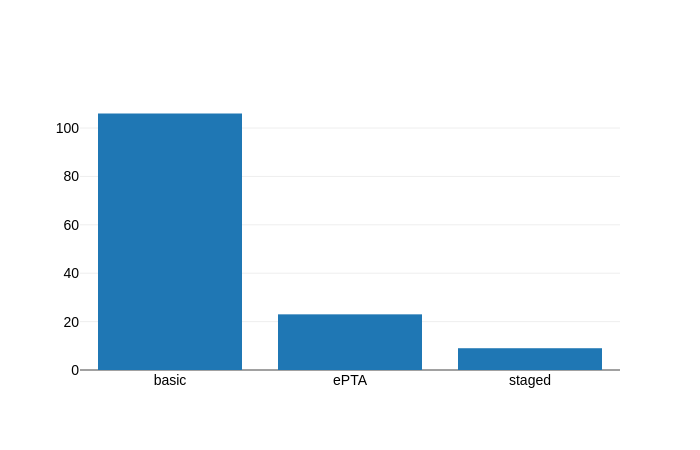
\includegraphics[width=\textwidth]{charts/bar_chart.png}
  \caption{The total increase of the number of instructions in \% when using
  the three configurations for the memory safety instrumentation.}
  \label{fig:increase_chart}
\end{figure}

\begin{table}[t]
\begin{tabular}{|l || r | r | r|}
 \hline
 & basic & ePTA & staged \\
 \hline
 \hline
 true     & 116 & 123  & 183 \\
 \hline
 false    & 132 & 133  & 135 \\
 \hline
 timeout  & 139 & 130  & 71 \\
 \hline
\end{tabular}
\caption{The numbers of \emph{true}, \emph{false} and \emph{timeout} answers
given by \symbiotic when using the three configurations for the memory safety
instrumentation.}
\label{tab:answers}

\end{table}

The reduced number of inserted instruction had indeed a positive effect on the
answers of \symbiotic as shown in Table~\ref{tab:answers}. When using the basic
approach, \symbiotic did not manage to decide 139 benchmarks in the given time
limit. With a pointer analysis, the number of timeouts slightly decreased. The
most significant improvement was achieved with the staged instrumentation:
\symbiotic ran out of time only in 71 cases. The both enhancements had impact
especially on the benchmarks that did not contain any violation of memory
safety.

We also measured the CPU running times of the instrumentation process. The
instrumentation using the basic approach took approximately 40~ms on average.
Even though the enhanced configurations of the instrumentation need to
additionally perform a pinter analysis at the beginning, the running times increased
insignificantly as showed in Figure~\ref{fig:times_chart}.

\begin{figure}[h]
  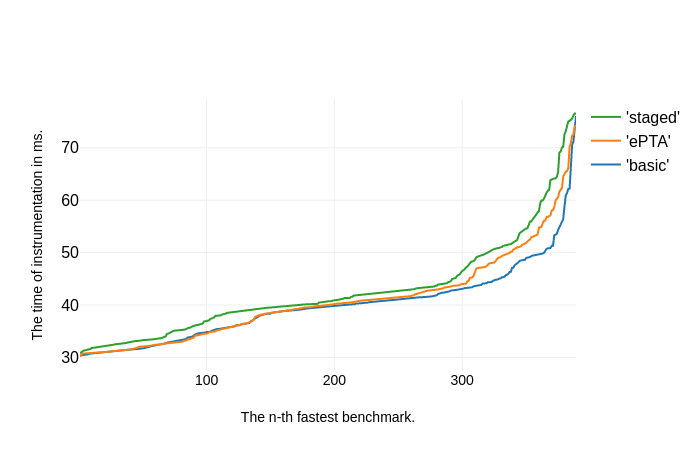
\includegraphics[width=\textwidth]{charts/instr_times_chart.png}
  \caption{The CPU running times of instrumentation when using
  the three configurations for the memory safety instrumentation.}
  \label{fig:times_chart}
\end{figure}



\chapter{Future Work}\label{chap:future}
In the future, we would like to implement a few more features to our
instrumentation tool. First fo all, we would like to enable not only insertion
of instruction, but also their replacement. This might seem a little bit
inconvenient at first sight, since the instrumentation is not supposed to
modify the given input program, however, a user might for example want to
replace calls of a function with calls of a function with the same semantics
but different implementation enriched with some analysis functionality, e.g.
logging.

Another improvement we would like to implement is insertion of more kinds of
instructions. As we mentioned earlier, inserting only \texttt{call}
instructions is sufficient, but we would like the tool to be as general as
possible.

Apart from the tool itself, we would also like to come up with new
configuration files for \symbiotic. Currently, we use \clang to check for
integer overflows in programs, but in the future, we want to create our own
configuration for the instrumentation to check for the overflows. This would
also lead to an implementation of a value analysis. \todo{dopsat}

As for memory safety configuration, we want to try replacing the lists for
preserving records with more efficient structure, such as trees.  \todo{jeste
neco?}


\chapter{Conclusion}\label{chap:conclusion}
Within this thesis, we listed tools that use instrumentation of LLVM~IR and
explained the need for a new tool for instrumentation that is not focused at
only one application, but is general and can be configured by user.

We implemented the tool such that it can be easily configured with two files
provided by user. Moreover, the tool can use results of other programs for
static analyses to get necessary information to reduce the amount of the
inserted code.

We also created a configuration for this tool that can be used to check memory
safety of programs. We improved this configuration by two enhancements: first,
we employed a pointer analysis to find out if it can itself decide whether a
pointer dereference is valid and then we divided the instrumentation into
stages to leave some of the memory allocations from the instrumentation. Both
of these enhancements led to a smaller amount of inserted code and therefore
faster analysis of the code.

Finally, we evaluated the configuration for checking memory safety by employing
the instrumentation to the tool \symbiotic and running it on a set of
benchmarks from SV-COMP.


\addcontentsline{toc}{chapter}{Bibliography}
\printbibliography

\appendix %% Start the appendices.
\chapter{An appendix}
Here you can insert the appendices of your thesis.


\end{document}

